\documentclass[12pt]{article}
\usepackage{fullpage}
\usepackage{graphicx, rotating, booktabs} 
\usepackage{times} 
\usepackage{fbb} 
\usepackage{natbib} 
\usepackage{indentfirst} 
\usepackage{setspace}
\usepackage{grffile} 
\usepackage{hyperref}
\usepackage{tikz-cd}
 \usetikzlibrary{cd}
\usepackage[export]{adjustbox}
\usepackage[most]{tcolorbox}
\usepackage{verbatimbox}
\usepackage{lscape}
\usepackage{afterpage}
\usepackage{amsmath}
\usepackage[labelfont={bf},textfont=it,labelsep=period]{caption}
 \usepackage{multirow} 
\setcitestyle{aysep{}}
\usepackage{dcolumn}

\hypersetup{
  colorlinks = true,
  urlcolor = blue,
  linkcolor = black,
  citecolor = black,
  pdfauthor = {Joshua Alley},
  pdfkeywords = {},
  pdftitle = {},
  pdfsubject = {},
  pdfpagemode = UseNone,
%  pdffitwindow = true
%  pdfcenterwindow = true
}



\singlespace
%\title{\textbf{Elections, Arms Deals and Autocratic Allies}}
\title{\textbf{Arms and Electoral Influence: How Arms Deals with Autocracies Shape Defense Contracting in the United States}}
\author{Joshua Alley \\
Assistant Professor \\
University College Dublin\thanks{Thanks to Brian Blankenship, Rosella Capella, Jonathan Caverley, Jonathan Chu, Ben Fordham, Erik Lin-Greenberg, Zachary Markovitch, Leah Matchett, Andy Philips and Phil Potter, as well as participants in the Boston University Political Economy of Security Online Workshop Series and 2022 Meeting of the International Studies Association for helpful comments.} \\
joshua.alley@ucd.edu
}

 
\date{\today}

\bibliographystyle{apsr}

\usepackage{sectsty}
\sectionfont{\Large}
\subsectionfont{\noindent\large\textit}
\subsubsectionfont{\normalsize}

\makeatletter
\renewcommand\tiny{\@setfontsize\tiny{9}{10}}
\makeatother


\begin{document}

\maketitle 

\begin{abstract} 
Arms deals with autocracies, especially allied states, increase defense contracting in U.S. swing states. 
U.S. leaders make arms deals to use defense contracts to improve economic conditions in pivotal electoral areas.
Autocratic security partners have the necessary combination of security need and political flexibility to strike arms deals near elections. 
I examine these claims by analyzing the electoral determinants of defense contracting and arms deals.  
First, I detail electoral cycles in arms deals between the United States and autocracies. 
I then link defense contract awards to swing states and arms deals.
Finally, I provide more fine-grained evidence of the mechanisms by showing that autocratic allies drive most of the deals cycle and that the same platforms that move in arms deals drive increased swing state contracts.  
The argument and results help explain why U.S. security cooperation with autocracies endures despite divergent regimes. 
\end{abstract} 


\newpage 
\doublespace 


\section{Introduction}



% US-Brazil 1972
In 1972, the Nixon administration struck ten deals to transfer or sell arms to Brazil.
Over the next four years, Brazil's military dictatorship received 500 M-113 armoured personnel carriers, five destroyers, seven submarines, and eight S-2E Tracker anti-submarine warfare aircraft.
These deals came while Nixon sought reelection and subsequent deliveries continued after his 1974 resignation. 


% Obama 2012
Something similar happened during the 2012 presidential election, when Saudi Arabia ordered arms from the Obama administration.\footnote{Obama first announced the deal in 2010.} 
Twelve deals included 400 Harpoon anti-ship missiles, 12 Apache attack helicopters for the Saudi National Guard, and 63 K-6 120mm mortars, along with parts for F-15 aircraft, guided bombs, and other helicopters. 
Deliveries of these systems and other weapons spanned the next eight years, including the 2015 Saudi intervention in Yemen's civil war.\footnote{All deal information from \citep{SIPRI2021}.}


% puzzle
Such extensive U.S. security cooperation with autocracies is somewhat puzzling.
Other countries and domestic elites often criticize U.S. support for autocrats as counterproductive and hypocritical. 
Autocracies may be less reliable partners \citep{Gaubatz1996} and cooperation in between democracies and autocracies can be brittle \citep{Leeds1999}, but the United States has made longstanding security ties with many autocracies.  


% example- PBC consequences vary w/ security coop
Despite the potential drawbacks of working with autocracies, electoral competition in the United States encourages arms deals with autocracies, especially autocratic allies.
Leaders make arms deals with autocracies to increase defense contracting as elections approach.
Greater defense contract awards concentrate in swing states, improving economic conditions in key regions and bolstering leaders' efforts to retain power \citep{Tufte1978, Mintz1988, Mayer1995, DerouenHeo2000, Becker2021}. 


% arms exports logic
Autocracies are a useful partner for electoral cycles in arms deals because autocrats have the security need and political flexibility to strike deals near elections. 
Unlike democratic leaders, who could face opposition criticism for making arms deals, autocrats have few constraints on accommodating electoral cycles.
Autocracies can then use arms to fortify their regime against external and internal threats.
These incentives are especially pronounced in alliance prot{\'e}g{\'e}s as autocratic U.S. allies rely on arms for security \citep{McManusYarhi-Milo2017}.
%These arms export cycles reinforce cooperative relationships between U.S. leaders and alliance prot{\'e}g{\'e}s. 


% Findings
I scrutinize my argument connecting defense contracting in swing states, autocratic allies and arms deal cycles in three steps. 
First, I analyze U.S. arms deals from 1950 to 2014, and show that arms deals with autocracies increase as presidential elections approach, while arms deals with democracies are unchanged. 
Second, I estimate the association between arms deals and contract awards to swing states, and find that arms deals have little association with contracts outside of swing states, but increase contract awards in swing states. 
Finally, I corroborate these correlations by examining the mechanisms in two ways.
The first mechanism check establishes that allied states drive most of the association between autocracies and electoral cycles, which shows the importance of autocratic security motivations. 
The second check shows that the weapons systems that cycle in arms deals are most correlated with more swing state contracts.


% focus on the U.S.
%The pivotal economic and security roles of the United States make understanding the economic and security consequences of U.S. electoral competition worthwhile. 
%The United States is the leading arms exporter, maintains expansive alliance ties, and there is prior evidence that leaders use defense contracting for electoral advantage \citep{DerouenHeo2000}. 
%Other states might leverage security cooperation to facilitate different policy cycles, however. 


% economic and seucrity ties 
The argument and findings address three salient issues in international relations theory and practice. 
First, they provide new insight into alliance bargaining and statecraft, and suggests one reason why U.S. alliances with autocracies endure. 
When arms deals with autocracies help U.S. leaders keep office, patron leader and prot{\'e}g{\'e} incentives align.
Work on alliance bargaining often examines coercion and divergent preferences \citep{WolfordKim2017, Resnick2019, Blankenship2020, Beckeretal2023}. % \citep[pg. 122]{Oatley2015}
But as \citet{Baldwin2020} notes, statecraft also includes positive inducements. 
This note highlights positive statecraft by alliance prot{\'e}g{\'e}s and connects with prior work on issue linkage in alliance management \citep{Davis2008, Poast2013}.
Electorally driven arms deals are an indirect way smaller partners influence alliance patrons \citep{Keohane1971}.


% value of autocratic allies
Second, this note reveals the electoral causes and consequences of security cooperation. 
Just as domestic political business cycles in large countries reshape economic conditions \citep{Kayser2006}, electoral competition alters security cooperation. 
Security cooperation has electoral ramifications as well. 


Finally, my results complement prior findings that foreign states' economic policies impact electoral competition. 
\citet{KimMargalit2021} find that Chinese tariffs reduced Republican vote share in the 2018 midterm elections by targeting industries in competitive districts.
In the same way, \citet{ChyzhUrbatsch2021} find that Chinese soy tariffs hurt Republican congressional candidates in soy-producing areas. 
My argument inverts these findings by considering how security cooperation provides ways to manipulate economic conditions. 


% need an outline 
The note begins by outlining the international consequences of political business cycles in the United States, the role of defense contracting in those cycles, and the consequences for arms deals with autocracies. 
I then test the theoretical process in three steps. 
First, I demonstrate that arms deals between the United States and autocracies increase as presidential elections approach. 
I then show that arms deals are correlated with increased defense contract awards to swing states.
Third, I examine the mechanism by analyzing autocratic allies and analyzing which weapons drive deals cycles and increased swing state contracts.
The last section discusses the results and offers concluding thoughts.


\section{Argument}


My argument claims that arms deals with autocracies facilitate defense contract awards in swing states.
To begin, I detail constraints on aggregate budget cycle tools.
I then discuss how presidential control and Congressional influence makes defense contracting an attractive way to manipulate economic conditions, and how arms deals can accelerate defense contracting awards. 
Finally, I explain why low constraints and high security need make autocracies willing to make arms deals around U.S. elections.


Electoral considerations impact policy \citep{Nordhaus1975}.\footnote{See \citet{Dubois2016} for a review of the vast political budget cycle literature.} 
When leaders want to win office, they can use policy tools to bolster economic growth and win over voters. 
Leaders create political budget cycles by using fiscal and monetary policy to increase economic growth near elections and retain power for themselves or their party \citep{Tufte1978, Rogoff1987}. 


The composition and magnitude of these cycles varies. 
Strong central bank interdependence and fixed exchange rates make fiscal cycles more likely, for instance \citep{ClarkHallerberg2000}. 
Federal Reserve independence limits political influence on monetary policy in the United States. 
In fiscal policy, aggregate budgets often constrain spending discretion.


Given challenges with using aggregate economic instruments, recent scholarship on political cycles emphasizes targeted policies.
Focused manipulations maximize the electoral impact of finite resources.
Many spending shifts can be narrowly tailored \citep[pg. 248]{Dubois2016}.
Leaders also employ other policies such as trade disputes \citep{Conconietal2017}, labor agreements \citep{Ahlquist2010} and land reform \citep{Philips2020} to win support in key constituencies.


% Defense spending/contracts as flexible instrument
Scholars have long speculated that defense spending is a useful instrument for budget cycles (e.g. \cite{Tufte1978, Mintz1988}).
Leaders often have more discretion in defense resource allocation, and defense spending impacts economic conditions.
\citet{WhittenWilliams2011} note that defense spending can serve social welfare goals and \citet{Becker2021} finds that unemployment encourages NATO members to shift spending from equipment to personnel.


% in US context, contracts
Studies of the United States argue that defense budgets are poor political tools, however, as Congress makes allocations two years ahead.
This shifted attention towards defense contracting, as leaders control contract timing and disbursement \citep{Mayer1995, DerouenHeo2000}.
Giving contracts also allows leaders to focus on key constituencies and claim credit for contract awards \citep{DerouenHeo2000}. 


In the United States, leaders target political spending changes to electorally important areas.
For presidents, swing states are the most important regions \citep{KrinerReeves2015}, as they hold the balance of the Electoral College. 
Such targeted spending support for incumbents \citep{KrinerReeves2012}.


% demand- stability
%The Congressional budget process sometimes hinders political contracting stability. 
%Leaders can allocate contracts within the budget, but finding additional funds is harder. 
%Most defense programs operate on annual budget allocations.
%Congress rarely authorizes multi-year procurement. % CITE CRS HERE 
%As a result, program disbursements can vary from year to year, especially for smaller outputs like munitions and missiles. 


Increasing contract awards also has limits, however. 
The defense budget constrains contracting levels. 
Also, if leaders want to award more contracts, the U.S. military may lack absorption capacity to incorporate outputs.
Political increases in supply of defense contracting may not respond to military demand.
This makes finding other buyers necessary.


Foreign markets are an alternative source of demand for defense goods.
Either foreign countries can take new production, or U.S. leaders can sell or transfer old equipment to partners to make room in U.S. stocks. 
When this occurs, using defense contracting for political gains has international spillovers.\footnote{% Political Business cyles
Other work examines the international economic consequences of budget cycles.
Economic interdependence leads to correlated economic growth across countries \citep{Kayser2006} and increases the global economic influence of large economies. 
\citet{Ito1991} finds that U.S. elections increase economic growth in Japan, while \citet{FoersterSchmitz1997} argue that U.S. electoral cycles impact international stock returns.
}


% timeline and intermediate goods
Leaders only need arms deals and confirmed orders to award contracts to electorally important areas.
Final transfers can and often do come years later. 
Arms deals are more likely to follow electoral cycles than transfers of finished defense goods, as production times vary widely. 
Large platforms like ships, tanks and warplanes can take years to assemble, while munitions and smaller platforms take less time. 


% additional production and foreign markets
%When defense production and planning diverge, foreign markets provide alternative takers for excess arms production from defense contracting cycles. 
When U.S. leaders attempt to use arms deals to stimulate defense contracting, not all countries are useful partners. 
While all states could make deals, some have similar budget and political constraints. 
Autocracies have the flexibility and need to make arms deals around elections, however.



\subsection{Arms Deals with Autocracies}


While many states could benefit from U.S. arms, autocracies are more likely to make arms deals near elections. 
Autocracies have greater means and motivation to make arms deals than democracies.
Autocratic leaders have fewer domestic political constraints, which increases their budget and policy flexibility. 
They also have stronger security motivations to use arms deals to improve relations with the United States, because arms transfers are central to U.S. security cooperation with autocracies.


% to work, allies must have pol  and budget flexibility
%Leaders must have the political freedom to make arms deals.
%Governments are the customer for most arms sales or transfers, so they generally have some latitude to take arms.\footnote{This mirrors how political control of firms increases trade policy flexibility \citep{Davisetal2019}.}
%At the same time, not every regime is equally free to make arms deals. 


% constraints
Autocracies have greater political flexibility to make arms deals around elections than democracies. 
Democratic leaders might face media or elite scrutiny of deals for U.S. arms.
Media or elites might object to spending on arms, competition for domestic arms manufacturers, or excessive alignment with the United States.
Democracies are also more likely to engage in joint production of weapons systems, due to domestic political benefits and closer ties with the United States.


% laws and budget processes
Democratic leaders also face the same budget constraints that encourage U.S. leaders to use defense contracting to manipulate economic conditions. 
Spending on U.S. arms is unlikely to help democratic leaders retain office. 
As a result, they will spend finite resources elsewhere. 


Autocrats are less constrained.
Even if other domestic actors in an autocracy are opposed to additional outlays on U.S. arms, they have few ways to constrain the leader.%\footnote{This changes when opponents of U.S. arms deals are part of the autocrats power base.}
Media scrutiny of deals is also less likely to occur or challenge an autocrats power base. 


% offstage signaling and need
Autocrats also strike deals to bolster their security.
Arms transfers are more central to U.S. cooperation with autocracies.  
The United States prefers ``offstage'' signals of support for autocrats, rather than public demonstrations of commitment \citep{McManusYarhi-Milo2017}.
Arms transfers are a pivotal offstage signal and can substitute entirely for formal security guarantees \citep{Yarhi-Miloetal2016}. 
When arms are essential to U.S. security commitments, autocrats will make deals that increase their military capabilities and signal continued alignment with the United States.
This mirrors how democracies can use aid to get foreign policy concessions from autocracies, but not democracies \citep{BDMSmith2009}.


% further need- no ideological affinity
Autocracies also have fewer other tools to curry favor with U.S. leaders.
Formalizing an informal alliance might promote democratization \citep{GiblerWolford2006}.
The U.S. public prefers security cooperation with democracies \citep{Alley2022}, so autocrats have less capacity to pursue deeper ties in other areas. 

% internal
Internal security concerns further motivate autocratic deal-making. 
Maintaining a robust coercive apparatus is essential to autocratic leaders' survival in office \citep{Boix2008}. 
U.S. arms can provide coercive capacity or allow leaders to invest more in repressive capabilities by substituting for other defense goods. 
Given these security needs and political flexibility, autocrats are more likely to make arms deals near elections.



% deliberate or not?- key for statecraft argument. 
This argument is agnostic about whether allies make a conscious decision to help political budget cycles by making arms deals.
While they want improve their alliance relationship, U.S. allies need not choose to accommodate electoral cycles in defense contracting.
Allies may receive better terms and more financial support to take additional goods, or take transfers or surplus materiel as a deliberate favor to U.S. leaders who support their foreign policy interests. 


% objection- more scrutiny of deals around elections
A potential objection to this argument is that striking arms deals with autocrats near elections is risky for U.S. leaders. 
Even if political opponents criticize deals, U.S. leaders may still benefit, as arms deals provide concentrated benefits.
More diffuse critics face collective action problems that reduce their influence.
When contracts from deals flow to electorally salient areas, leaders will expect that deal benefits outweigh any costs. 



\subsection{Implications}


The argument generates two testable implications about U.S. arms deals and defense contracting. 
Again, this argument applies exclusively to the United States.  
Arms deal cycles and defense contracting in swing states are the result of a large defense industry and the Electoral College. 
Fixed election scheduling further reduces endogeneity between policy decisions and election timing. 
Other leaders may behave in similar ways within their electoral institutions, however. 


The first hypothesis predicts electoral cycles in arms deals, especially to autocracies.
Democracies will be less likely to make cyclical arms deals. 
As a result, greater proximity to presidential elections will increase arms deals with autocracies states. 


\begin{quote}
\textsc{Arms Deals Hypothesis: As time to a presidential election decreases, U.S. arms deals with autocracies will increase.}
\end{quote}


Second, I expect that arms deals increase contract awards in swing states.
Striking deals allows leaders to award contracts to electorally competitive areas. 
Winning swing states is necessary for retaining control of the executive branch. 
Outside of swing states, arms deals are less likely to increase contract awards. 


\begin{quote}
\textsc{Deals and Contracts Hypothesis: As arms deals increase, swing state contract awards will increase.}
\end{quote}


% What's next
Next, I examine both hypotheses. 
In the first analysis, I test the arms deals hypothesis with data on U.S. arms deals from 1951 to 2014.  
The second analysis tests the deals and contracts hypothesis with state-level defense contracting data from 2000 to 2020. 
Finally, I check the mechanisms by showing that autocratic allies drive the arms deal results and establishing that the defense industrial sectors with clear arms deals cycles also have the strongest association between deals and contracts. 


\section{Arms Deals and Presidential Elections}


The arms deals hypothesis predicts electoral cycles in U.S. arms deals with autocratic allies.
To test this hypothesis, I model U.S. arms deals from 1951 to 2014 using deals data from the SIPRI Arms Transfer Database \citep{SIPRI2021}.
The outcome in this panel dataset of all states outside the United States is the annual count of deals, based on SIPRI's trade register.\footnote{SIPRI's trade register captures individual transfers of specific platforms, and marks deal start, years of delivery, and deal completion.}
This section presents count data regression estimates of annual arms deals. 


% Why focus on deals
I analyze arms deals rather than observed arms transfers for three reasons.
First, elites can announce arms deals and related contracts immediately. 
Secondly, deliveries can take years after a deal is announced, even for second-hand or aid transfers of existing equipment. 
Finally, deliveries often space out the total value of a shipment over several years, especially for deals with many weapons or larger platforms. 


% key independent variables- ally/partner, 
The argument claims that election timing and partner regime interact to shape U.S. arms deals. 
I measure election timing and competition with an indicator of the number of years to a presidential election. 
As years to an election decrease, electoral competition increases. 


Next, I measure recipient democracy using the VDem project's polyarchy measure \citep{Coppedgeetal2008}. 
Polyarchy provides a fine-grained summary of democratic institutions and contestation.
It also suggests that Saudi Arabia, Iran, and Latin American juntas are among the most autocratic U.S. security partners, so it has some face validity.  


% models
Because many countries make no arms deals, I use a hurdle Poisson model to estimate how the interaction of democracy and election timing shape arms deals.\footnote{Standard Poisson models under-predict zeros, while negative binomial models predict over-predict large values. See the appendix for details.} 
The hurdle component captures that some countries are unlikely to make any arms deals, and fits the annual count of arms deals well.
For ease of estimation and calculation, I use Bayesian estimation with the brms package for \textsf{R} \citep{Buerkner2017}. 
I show in the appendix that Gaussian, Poisson and zero-inflated Poisson models give similar inferences. 


I adjust for other factors that are correlated with arms deals and partner democracy. 
One key factor is whether a country is a U.S. ally. 
I measure alliance status with a binary indicator of whether a country is a formal U.S. treaty ally using data from the ATOP project \citep{Leedsetal2002}.
I also include three states with inconsistent formal treaty commitments that are widely seen as U.S. allies; Israel, Taiwan and Saudi Arabia. 
I include informal allies because in some of these cases arms substitute for a formal alliance, but the United States is still supporting a partner's security \citep{Yarhi-Miloetal2016}. 
%All three countries with informal alliances have implicit security guarantees that are similar to U.S. treaties with other countries. 


Two other control variables are binary indicators of Cold War years and peak years in the Global War on Terror, as the United States had more autocratic partners during these periods. 
I also adjust for EU membership as a potential constraint. 
Further country-year level controls include militarized dispute involvement, logged GDP, population, and distance from the United States, as well as a binary indicator of common language. 
Finally, I adjust for presidential partisanship with a dummy indicator of Republican administrations.  


In the hurdle equation of the model, I use four predictors to capture whether a country will make any arms deals with the United States. 
First, I include the binary indicator of alliance status and the polyarchy democracy measure, because autocracies and non-allied states are less likely to make arms deals. 
I also include an indicator of whether a country is engaged in an active militarized dispute. 
Finally, I include the log of GDP, because wealthier countries have greater means to buy U.S. arms.\footnote{The regression coefficients use a normally distributed prior distribution and a mean of zero and standard deviation of .5.}


\subsection{Results}


I summarize the interaction of partner democracy and presidential election proximity in \autoref{fig:democ-deals-pred}.\footnote{See the appendix for coefficient estimates from all models.}
This figure plots predicted arms deals based on proximity to a presidential election and partner democracy.
Each facet fixes recipient democracy at the minimum, first quartile, median, third quartile and maximum.


\begin{figure}[htpb]
	\centering
		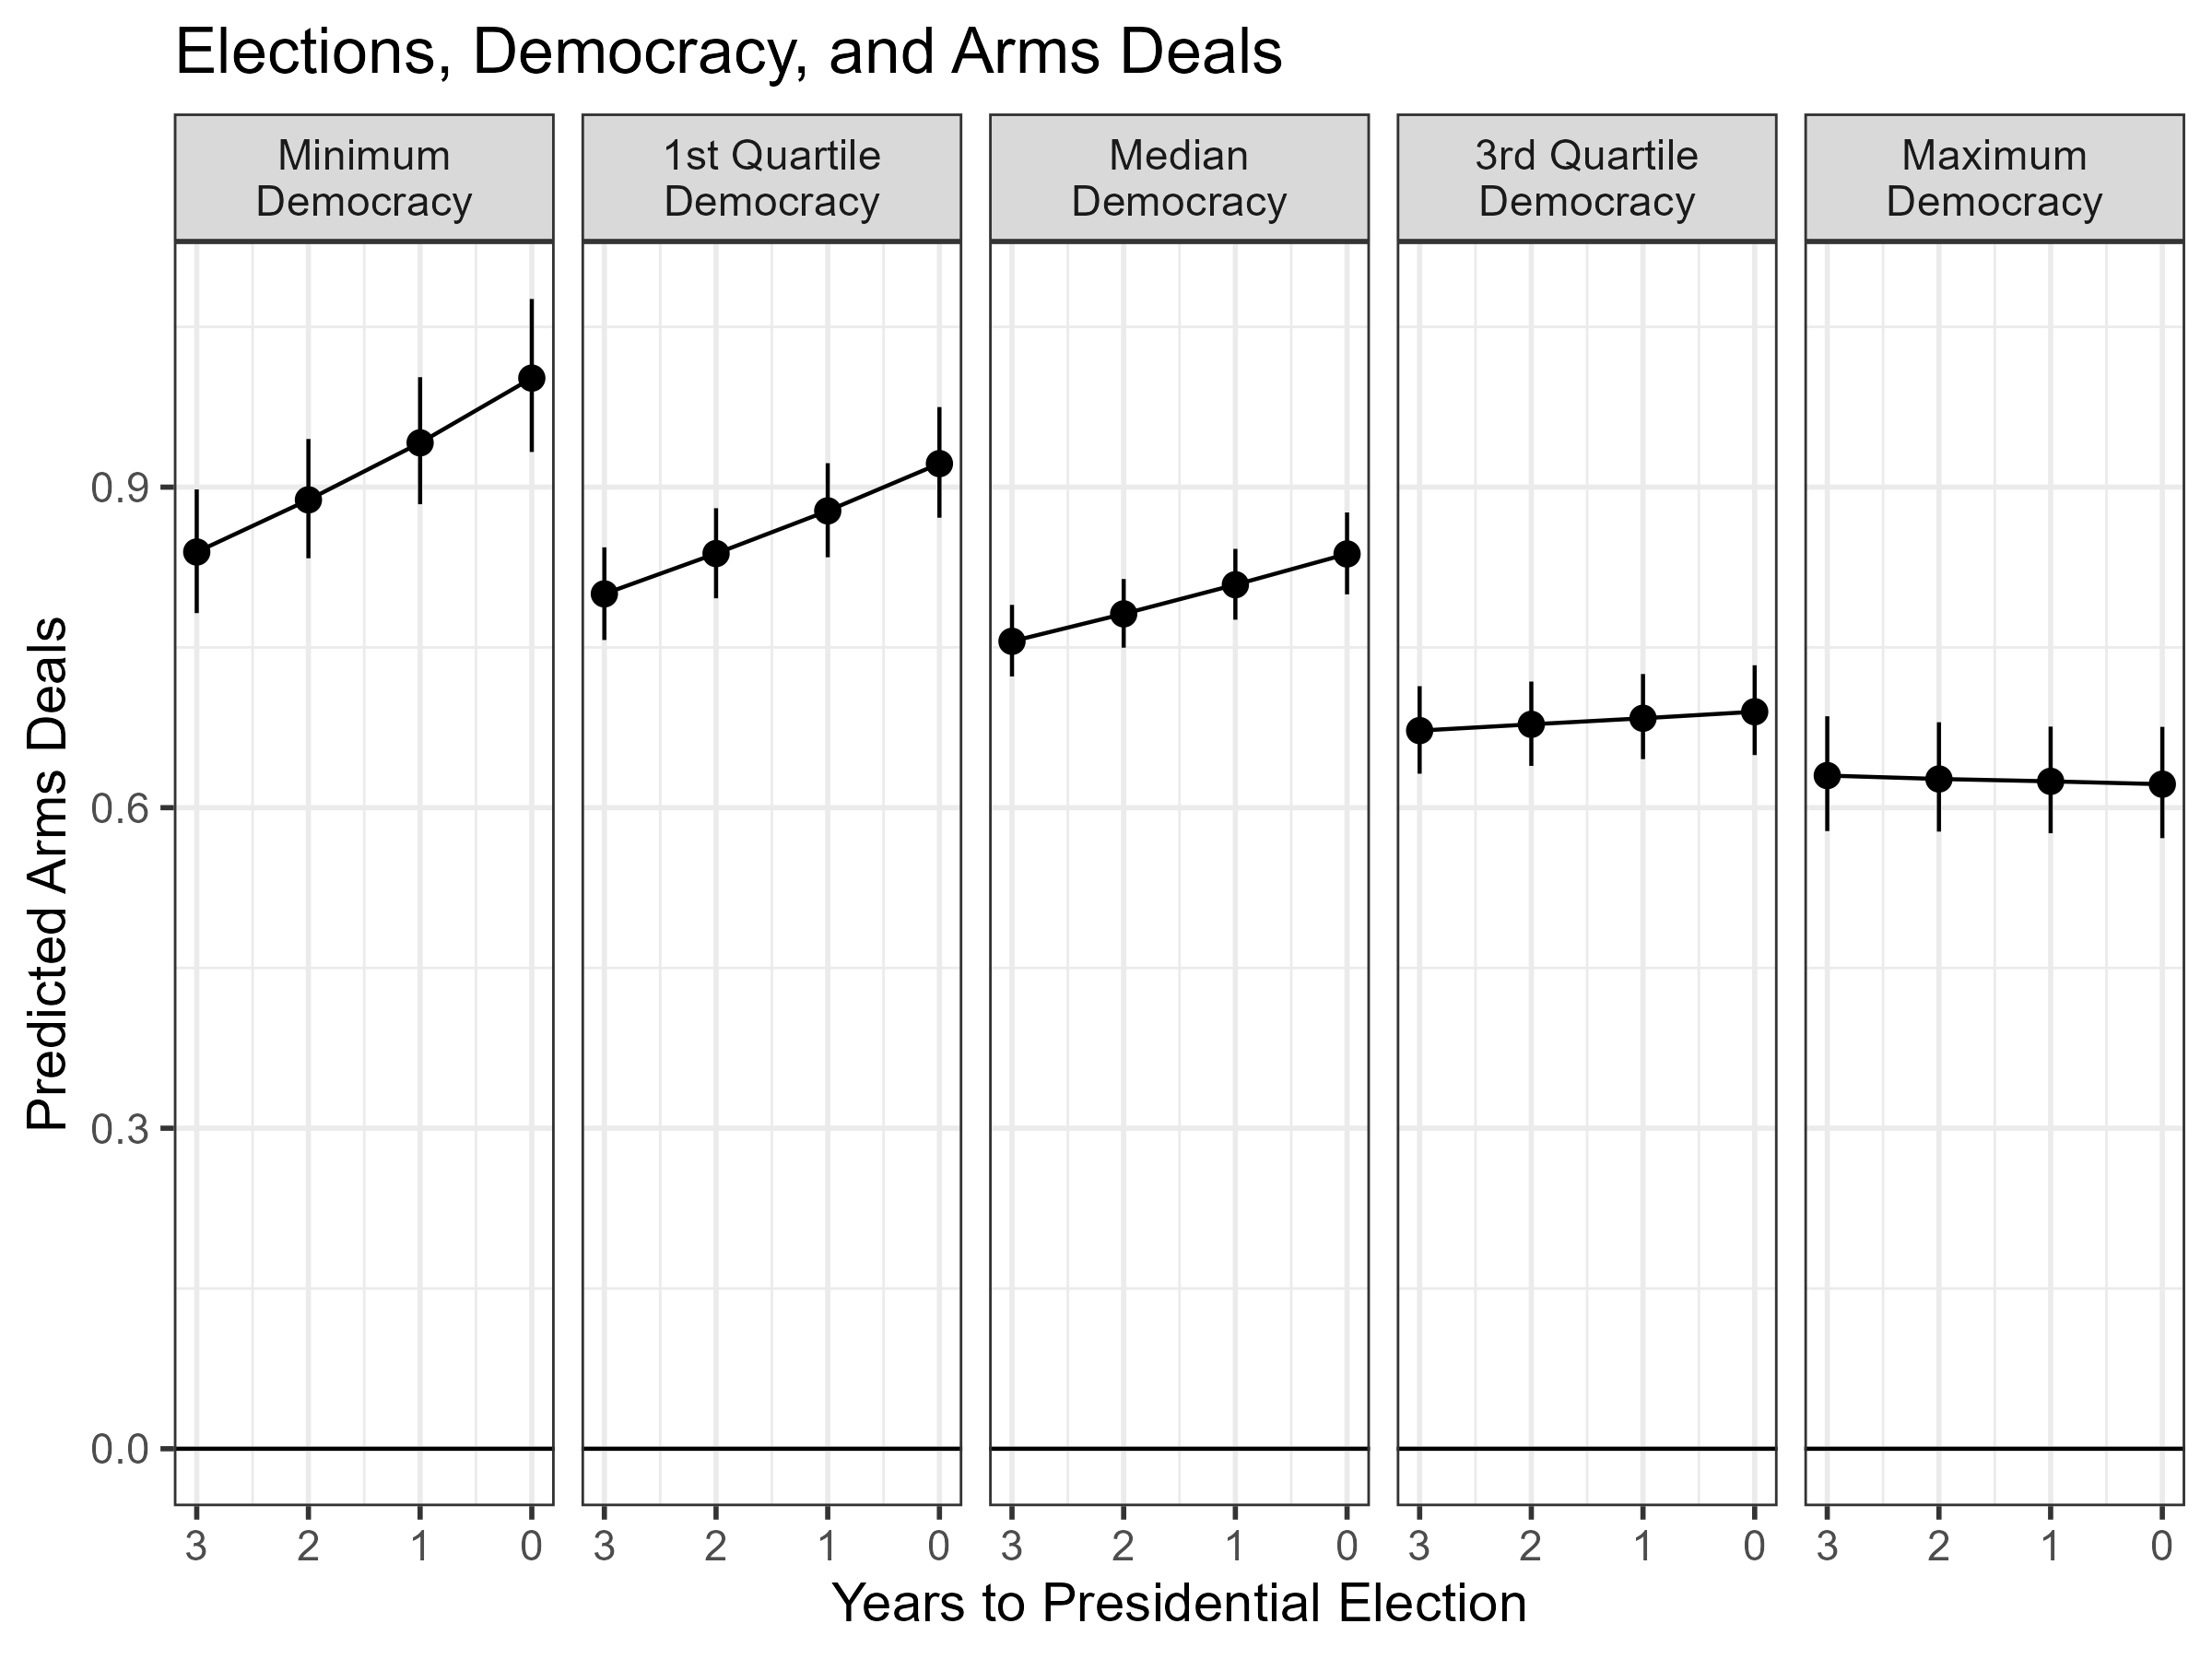
\includegraphics[width=0.95\textwidth]{../figures/democ-deals-pred.png}
	\caption{Predicted arms deals between the United States and other states 1950 to 2014 based on presidential election proximity and partner democracy. Estimates derived from a hurdle Poisson model. Points mark the estimates and error bars summarize the 90\% credible interval.}
	\label{fig:democ-deals-pred}
\end{figure}


\autoref{fig:us-arms-plots} indicates that electoral cycles in arms deals are present for autocracies allies and absent for democracies.
At minimum polyarchy, predicted arms deals rise from .84 to 1 throughout the presidential election cycle.
Hypothesis tests of equality between allied arms deals at minimum democracy at each level suggest that the increase of .06 deals in each year of the electoral cycle is is clearly positive.\footnote{The entire posterior mass of the difference between three and zero years to an election is positive, with a 90\% credible interval that ranges from .1 to .22.}
The electoral cycles when democracy is at the 1st quartile or median are also clearly positive, but smaller.
This cycle diminishes as democracy increases, so states with a polyarchy score at the third quartile or higher see no change in arms deals as elections approach.  


Furthermore, predicted arms deal levels increase as polyarchy decreases. 
This further supports expectations that autocracies who receive arms from the US are more interested in making these deals that democracies. 
Autocracies have different constraints and security concerns. 


As presidential elections approach, arms deals with autocracies rise. 
Arms deals with democracies are unchanged by electoral competition.
These arms deals with autocracies near elections are connected to defense contracting in swing states. 
The next analysis examines the deals and contracts connection.


\section{Arms Deals and Defense Contracting}


% describe the model 
Connecting arms deals and defense contracting is challenging. 
Deals occur between countries, while defense contracting for electoral advantage takes place within US states.
While jointly modeling deals and contracts is theoretically possible, summing country-year deal estimates into an annual measure of total deals creates an aggregation problem. %\footnote{A time-series model of aggregate defense deals could address this problem, but it would not show regime differences in arms deals.}
In the interest of simplicity, this analysis uses observed annual deals, electoral competition and state-level factors to predict defense contract awards from 2001 to 2020. 


I draw the outcome measure from Department of Defense prime contract award data in the USAspending.gov database.\footnote{Link here: \url{https://www.usaspending.gov/download_center/custom_award_data}.} 
This archive contains individual contract awards from 2000 to 2020.\footnote{I analyze defense contracting in these years because archive starts in the 2000 fiscal year and some state-level controls have limited coverage after 2020.}
While other contracts datasets have longer temporal coverage, they are less detailed.
I use the individual contracts data because it provides necessary detail to examine the role of electoral geography, and later to link arms deals and contracts in defense industry sectors. 


The key outcome is total defense contracts awarded to each state every year, measured in millions of US dollars.
I focus on contracts for arms production, because arms deals should have little impact on contracts for things like construction equipment or food.
While connecting specific contracts to foreign military sales is challenging, the narrow focus on arms production and subsequent analysis matching weapons systems and contracts mean that this approach still provides a useful test. 


Total defense contracts are also challenging to model, because some states have no weapons contract awards in a given year, and other states receive billions of dollars in contracts. 
The resulting outcome is zero-valued and right-skewed. 
Transformations of such data can make calculating substantive effects challenging and potentially biased. 
Traditional approaches such as logging the outcome after adding one are sensitive to the outcome scale and the constant added \citep{ChenRoth2022, MullahyNorton2022}. 


To overcome these issues, I fit two types of models.
First, I rescale the defense contracts measure to fall between zero and one by expressing each state's contracts as a share of total defense contracting in that year.
I then use ordered beta regression to predict the rescaled outcome \citep{Kubinec2022}.\footnote{\url{https://www.robertkubinec.com/post/logs/}} 
This allows me to use a flexible outcome distribution, account for zeros and avoid scale-effects from log-transformations and working with outcomes in millions of dollars. 
Changing the coefficients and marginal effects to the scale of contracts after this is straightforward, as I simply multiply the model estimates by the rescaling constant.
I also fit a a hurdle lognormal model of contracts without any transformation and a robust regression of annual contract changes. 
Both approaches give similar inferences.\footnote{See the appendix for results. All estimation uses brms for \textsf{R} \citep{Buerkner2017}.} 


The key independent variable is total annual arms deals.  
To measure arms deals, I sum US arms deals with all countries in every year. 
Annual deals range from 75 to 160. 


Because the argument expects that deals drive contracts in areas with high electoral competition, I include a dummy indicator of swing state status from \citet{KrinerReeves2015}.
Swing states are states where the losing party won at least 45\% of the two-party vote in three straight elections. 
I then interact this dummy with total US arms deals. 
My argument expects that the constituent term of arms deals, which expresses the association between deals and contracts outside of swing states, should be close to zero or negative.
Because there are no years with zero US arms deals, the swing state constituent term is not directly meaningful.  
The interaction term for swing states and annual deals should be positive, according to the deals and contracts hypothesis.


In addition to the electoral competition and deals variables, I include several controls. 
First, I adjust for population and GDP, because larger and more prosperous states receive more contracts. 
Other electoral competition indicators include the time to a presidential election and whether a state is a core member of the president's coalition \citep{KrinerReeves2015}. 
I also control for increased defense contracting demand during peak years in the global war on terror with a dummy variable that is equal to one from 2001 to 2011. 
The final control adjusts for presidential partisanship by coding years with a Republican President with one. 


Further adjustments in the model account for the data structure.
First, I include state varying intercepts because observations cluster within states. 
Current contracting also depends on past contracting, as the defense industrial base concentrates in particular states. 
I therefore include a state-specific lagged dependent variable, which allows temporal dependence in contracting to vary by state.\footnote{See the appendix for a summary of the state-level parameters.}


%Formally, the state-level equation is: 
%\begin{equation}
%\mu_{st}^{cont} = \alpha_{state} + \theta_s y_{st-1} + \rho_1 \mbox{Deals} + \rho_2 \mbox{Swing} + \rho_3 \mbox{Deals} * \mbox{Swing} + \textbf{G} \lambda
%\end{equation}


%This model is a useful test of the second hypothesis, as it assesses the impact of arms deals on swing states while adjusting for clustering, temporal variation and other predictors.
%The next section summarizes the estimates. 


\subsection{Results}


Because one of the interaction coefficients has no substantive meaning, I focus on marginal effects and predicted outcomes.
In \autoref{fig:deals-swing-me}, I present the impact of deals, swing state competition, and predictions from the interaction.
All these estimates suggest that deals increase defense contracting awards to swing states. 
To examine the conditional effect of deals, I use the positive posterior mass of the interaction term, because the deals and contracts hypothesis is directional.\footnote{For all other intervals, including the marginal effect of swing status and outcome predictions, I again use 90\% credible intervals, because these are less sensitive to simulation variance.}


First, the impact of increasing arms deals on defense contracting is unclear outside of swing states, but clearly positive in swing states. 
Only 34\% of the posterior mass in the deals constituent term is positive, so there is little evidence that deals increase contract awards outside of swing states. 
Full 98\% of the posterior mass of the deals and swing state interaction is positive, however. 
The preponderance of evidence supports the deals and contracts hypothesis.


\begin{figure}[htpb]
	\centering
		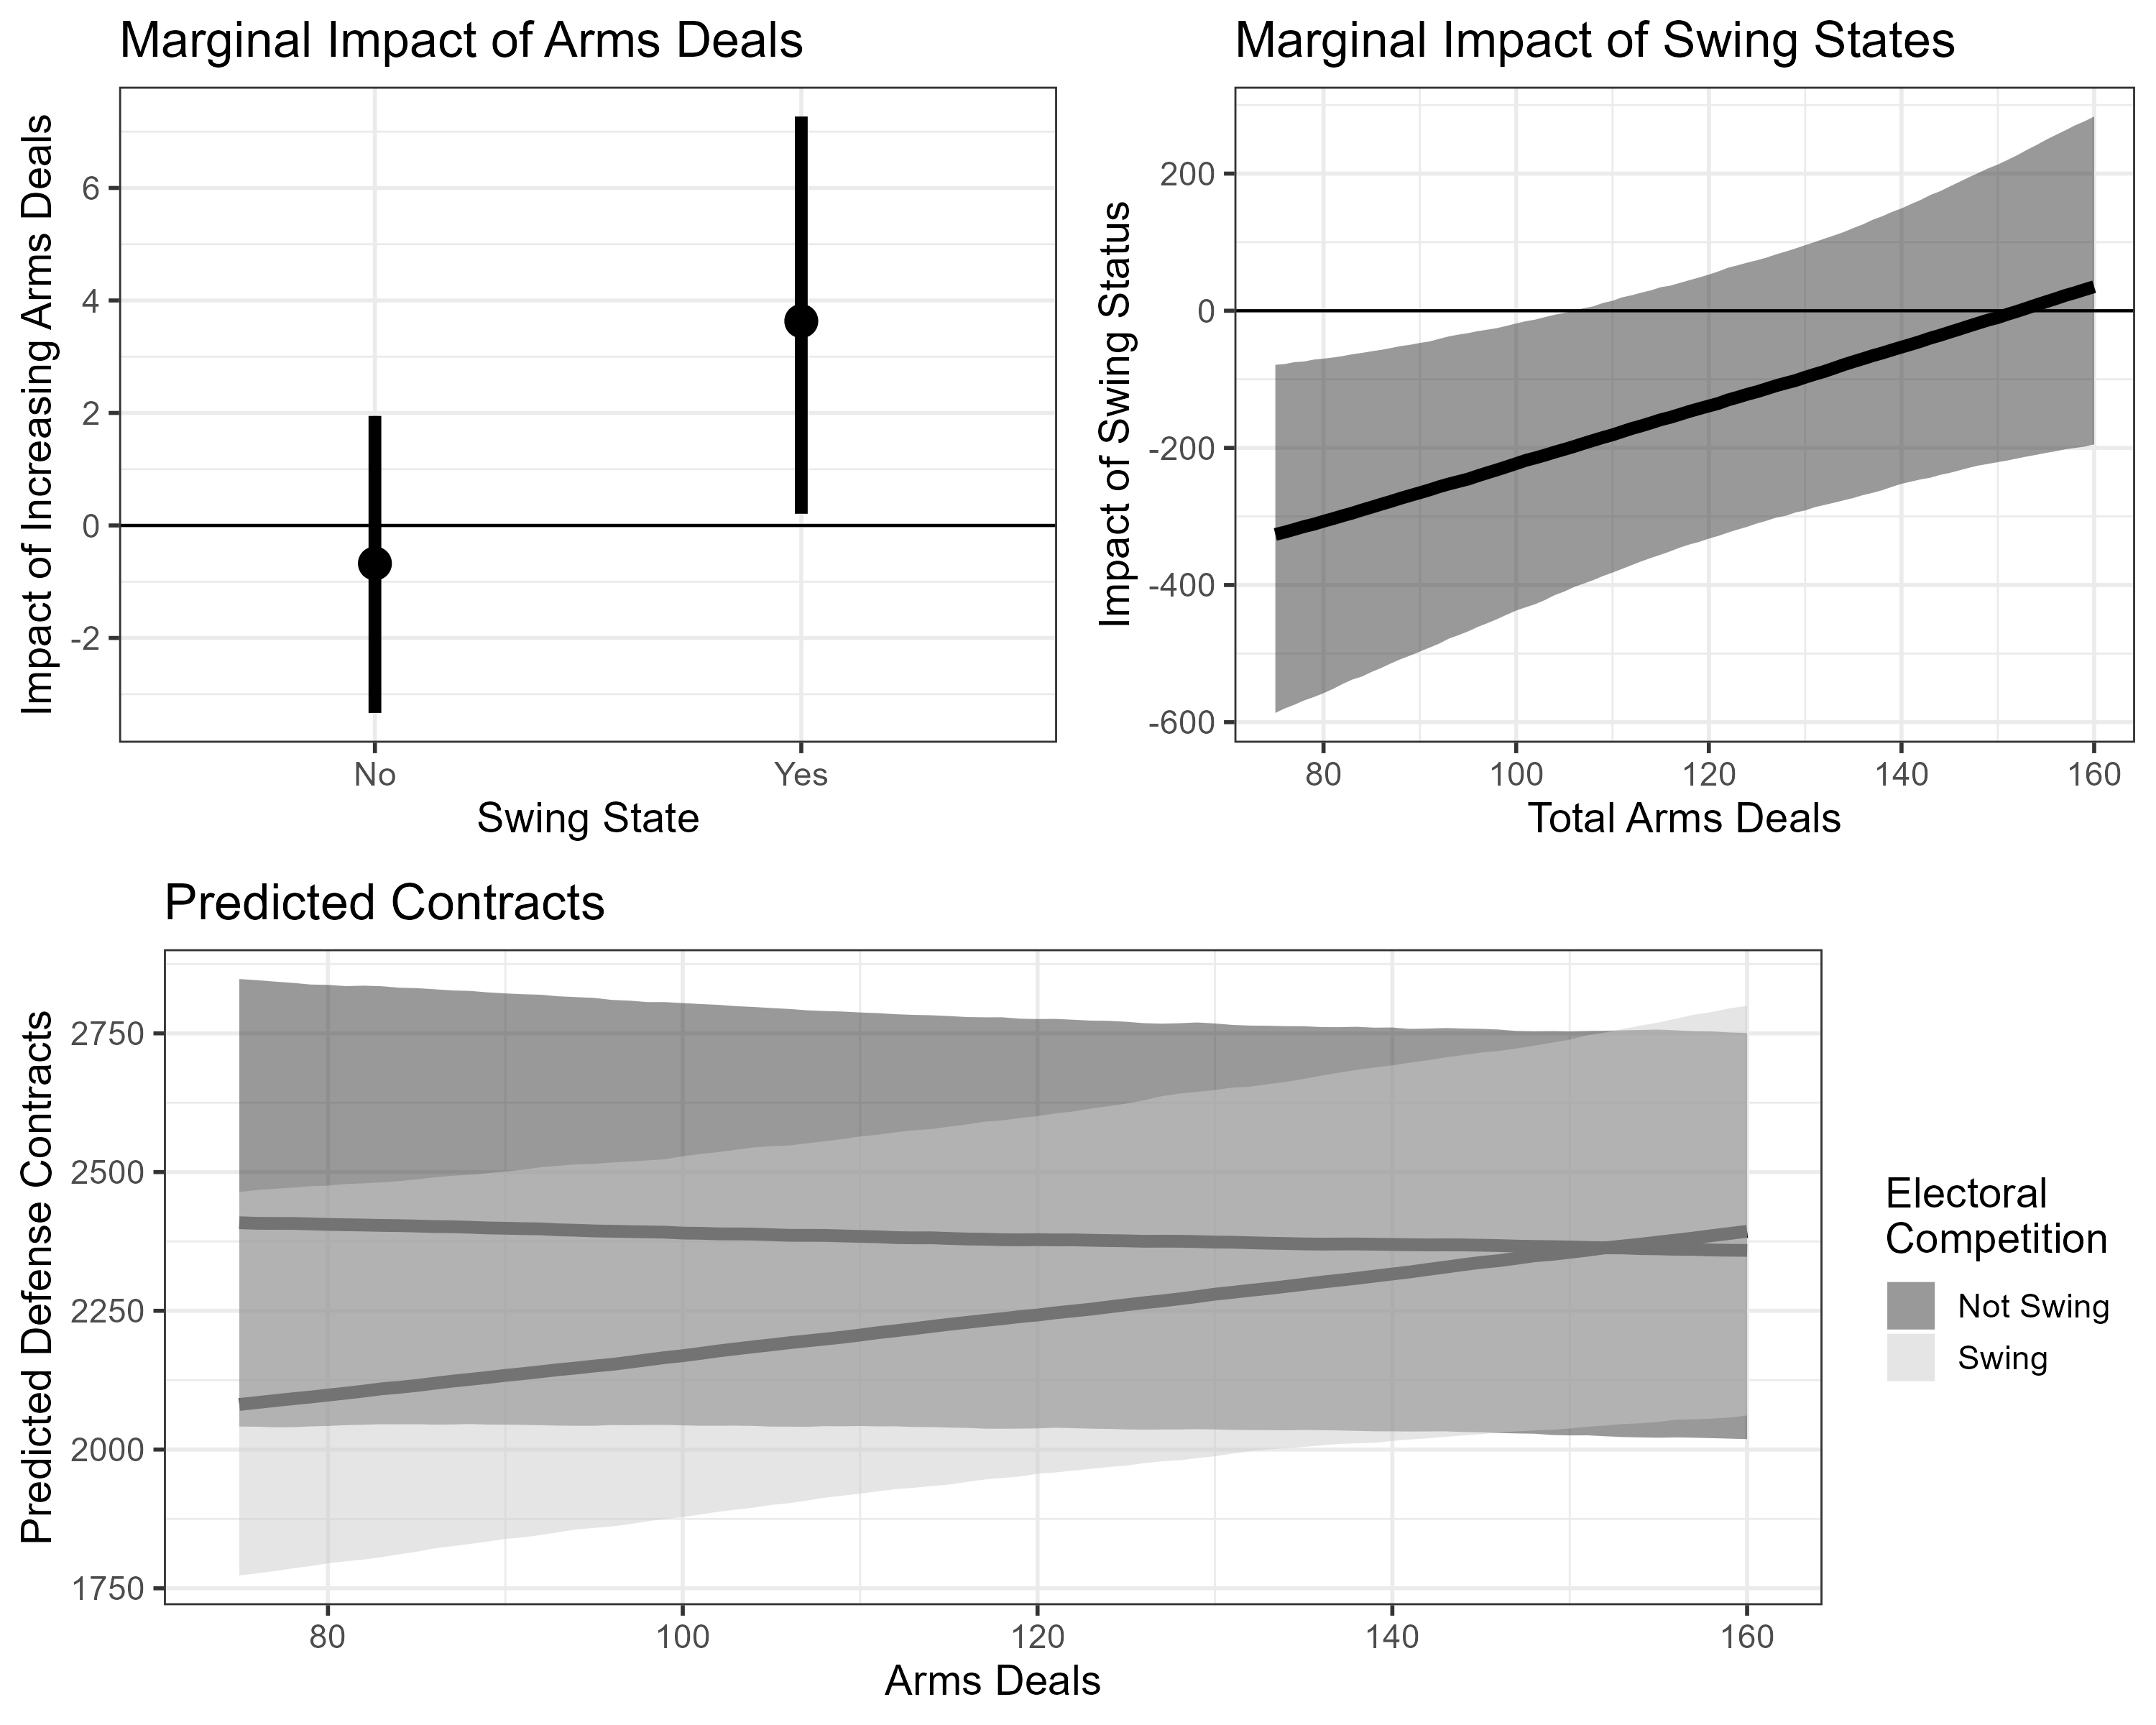
\includegraphics[width=0.95\textwidth]{../figures/deals-swing-me.png}
	\caption{Interaction coefficients, marginal effects and predicted outcomes from an interaction of swing state status and US arms deals. The outcome is annual defense contracts in the 50 US states from 2001 to 2020, measured in millions of dollars. Lines give the expected value, while the error bars summarize 90\% credible intervals. All other variables fixed at the mode or median.}
	\label{fig:deals-swing-me}
\end{figure}


The coefficient estimates in \autoref{fig:deals-swing-me} imply that moving from the first to the third quartile of deals increases defense contracting by \$202 million in a swing state, all else equal. 
Greater deals marginally decrease contract awards outside swing states because the share of contracts that go to swing states rise in election years. 
Leaders can thus use arms deals to target critical constituencies.


Second, swing states receive more defense contracts as arms deals rise. 
At the observed minimum of arms deals, swing states receive \$2.5 billion less in contracts.
The initial swing state disadvantage occurs because non-swing states like California and Texas have substantial defense industries.
When arms deals are near the observed maximum, swing states receive similar contracts to other states. 


Finally, predicted defense contracts increase as arms deals increase, but only in swing states, as the bottom panel of \autoref{fig:deals-swing-me} shows. 
Holding all else equal, increasing arms deals lead to greater contracts in swing states. 
But defense contracts in non-swing states do not respond to increasing arms deals.
As a result, the usual gap in defense contracting between swing and other states disappears in years with above-average arms deals. 



These estimates support the defense contracts hypothesis. 
Increasing arms deals are correlated with greater defense contracts in swing states. 
As a result, swing states receive similar contracts to other states with established defense industries, larger economies and less electoral competition. 
%Next, I use these estimates and the model of arms deals to estimate how much electoral cycles in arms deals with US allies add to defense contracting levels in swing states.  
%
%
%\subsection{Calculating the Defense Contracting Consequences of Arms Deals with Autocratic Allies}
%
%
%The following calculation is necessarily rough, as I combine predictions from two separate models. 
%To give a sense of how much defense contracting in swing states is due to arms deal cycles, I use predictions from hypothetical and observed data.
%Both these suggest that the increases in arms deals captured in \autoref{fig:us-arms-plots} are a substantively meaningful contributor to defense contracting in swing states. 

%
%Given these marginal effects, calculating the partial impact of alliances and allied regimes on deals and ultimately contracts is straightforward. 
%Across the electoral cycle with eight hypothetical countries of varying democracy and alliance status in \autoref{fig:democ-deals-pred}, there is one more arms deal in the election year, compared to the year after an election. 
%The marginal effect of arms deals is \$3.6 million, so the hypothetical cycle in deals and contracts adds several million in defense contracting to one swing state. 
%%
%
%These partial equilibrium associations are simple, but they may somewhat understate the impact of arms deals. 
%Because almost all defense production of finished and intermediate goods spans the United States, arms deals affect multiple swing states. 
%I therefore use predictions from observed data to assess the substantive impact of increasing arms deals. 


\section{Examining Mechanisms}


The above estimates corroborate two pieces of the argument, but require additional explanation. 
In the following, I check the mechanisms of low constraint and high security motivation by showing that autocratic allies drive most of the electoral cycle in US arms deals.  
Allies have the strongest security motivation to make arms deals and are the most likely autocrats to receive U.S. arms. 

After examining the role of alliances in arms deals cycles, I establish that the same platforms in arms deals between the United States and autocratic allies are also strongly correlated with swing state contracts.
If the platforms that moved in deals were uncorrelated with swing state contracts, that would suggest any connection between deal cycles and swing state contracts is purely coincidental.
The sectoral consistency I find instead suggests that arms deals do translate into swing state contracts. 



\subsection{Autocratic Allies}


% mechanisms
The argument claims that autocracies make arms deals with the United States near elections because their leaders have fewer constraints and reap security benefits. 
The confluence of need and freedom to make deals are both necessary for arms deals. 
Autocratic allies of the United States have similar political flexibility, but much greater security need. 
As a result, allied states should drive most of the electoral cycle in autocratic arms deals.\footnote{I focus here on formal and informal allies, because formal treaties like NATO are not the only U.S. security commitments.}


% potential markets: allies
% take new or used stuff to make room
Alliances increase arms transfers in general. 
\citet{Thurneretal2019} find that while the relative importance of security and economic factors fluctuates, alliances consistently increase arms transfers.
%Common security interests and defense industrial cooperation create economic and security ties that encourage arms trade \citep{Bitzinger1994}. 
\citet[pg. 184-5]{IkenberryGrieco2003} note that states often use direct transfers to attract and sustain security commitments. 
U.S. allies that rely on American weapons, systems and doctrines can also integrate new weapons more easily and make new deals that build on past orders. 


% security need
Autocratic allies also have more security need than democratic allies to accommodate electoral arms deal cycles. 
Winning favor with U.S. leaders increases the odds of U.S. support for an ally's foreign policy goals and domestic political survival.  
In addition to the capability boost of new arms, allies gain confidence in their patron's commitment when deals become deliveries because arms exports are a costly signal \citep{McManusYarhi-Milo2017}.


% less export cycles to non-allies
% each evidence sentence could be its own paragraph 
The security externalities of arms transfers reduce electoral cycles in arms exports to non-allies. 
U.S. leaders will be less willing to increase the capability of states with fewer common interests, even if it facilitates contracting cycles.
Justifying deals is more straightforward for autocratic allies. 



%Other U.S. elites are also more likely to object to arms deals outside alliances.
%Leaders could suffer electoral costs if other elites publicly criticize deals \citep{Saunders2022}.
%Arms transfers to non-allies could face greater opposition scrutiny near elections, leading presidents to forestall criticism by forgoing contentious transfers.
%Limited defense industry cooperation further constrains exports outside alliances, while allies with defense industrial ties can receive intermediate goods as well.


% Sales and transfers- who pays for what
%Moreover, prot{\'e}g{\'e}s do not always pay for U.S. arms.
%The United States often subsidizes or gifts arms transfers through foreign military sales programs. 
%While these still count as arms exports, they impose few immediate costs on recipients.
%Alliances make such subsidized transfers easier to justify to other elites, as they promote common security interests. 


% sum it up
Among autocracies, U.S. allies have stronger security motivations to take arms, along with the same lack on constraint as other autocracies. 
Allied states thus have the means and ample motivation to buy arms near elections. 
Alliances also make it easier for U.S. leaders to justify deals.
As a result, most of the electoral cycle in arms deals with autocracies is driven by allied states. 
 

 
\subsubsection{Results}

To examine the role of alliances, I modify the model of autocracies and electoral arms deals.
Specifically, I interact the dummy indicator of whether a state is a U.S. ally with the interaction of partner regime and presidential election proximity. 
This creates a triple interaction of alliance, regime type, and election timing. 


Because interpreting coefficients in triple interactions is challenging, I summarize the interaction of alliances, democracy and presidential election proximity in \autoref{fig:us-arms-plots}.
This figure plots predicted arms deals based on proximity to a presidential election, democracy and whether a state is a U.S. ally or not. 
Each facet divides estimates based on democracy, while colors distinguish between allied and non-allied states. 


\begin{figure}[htpb]
	\centering
		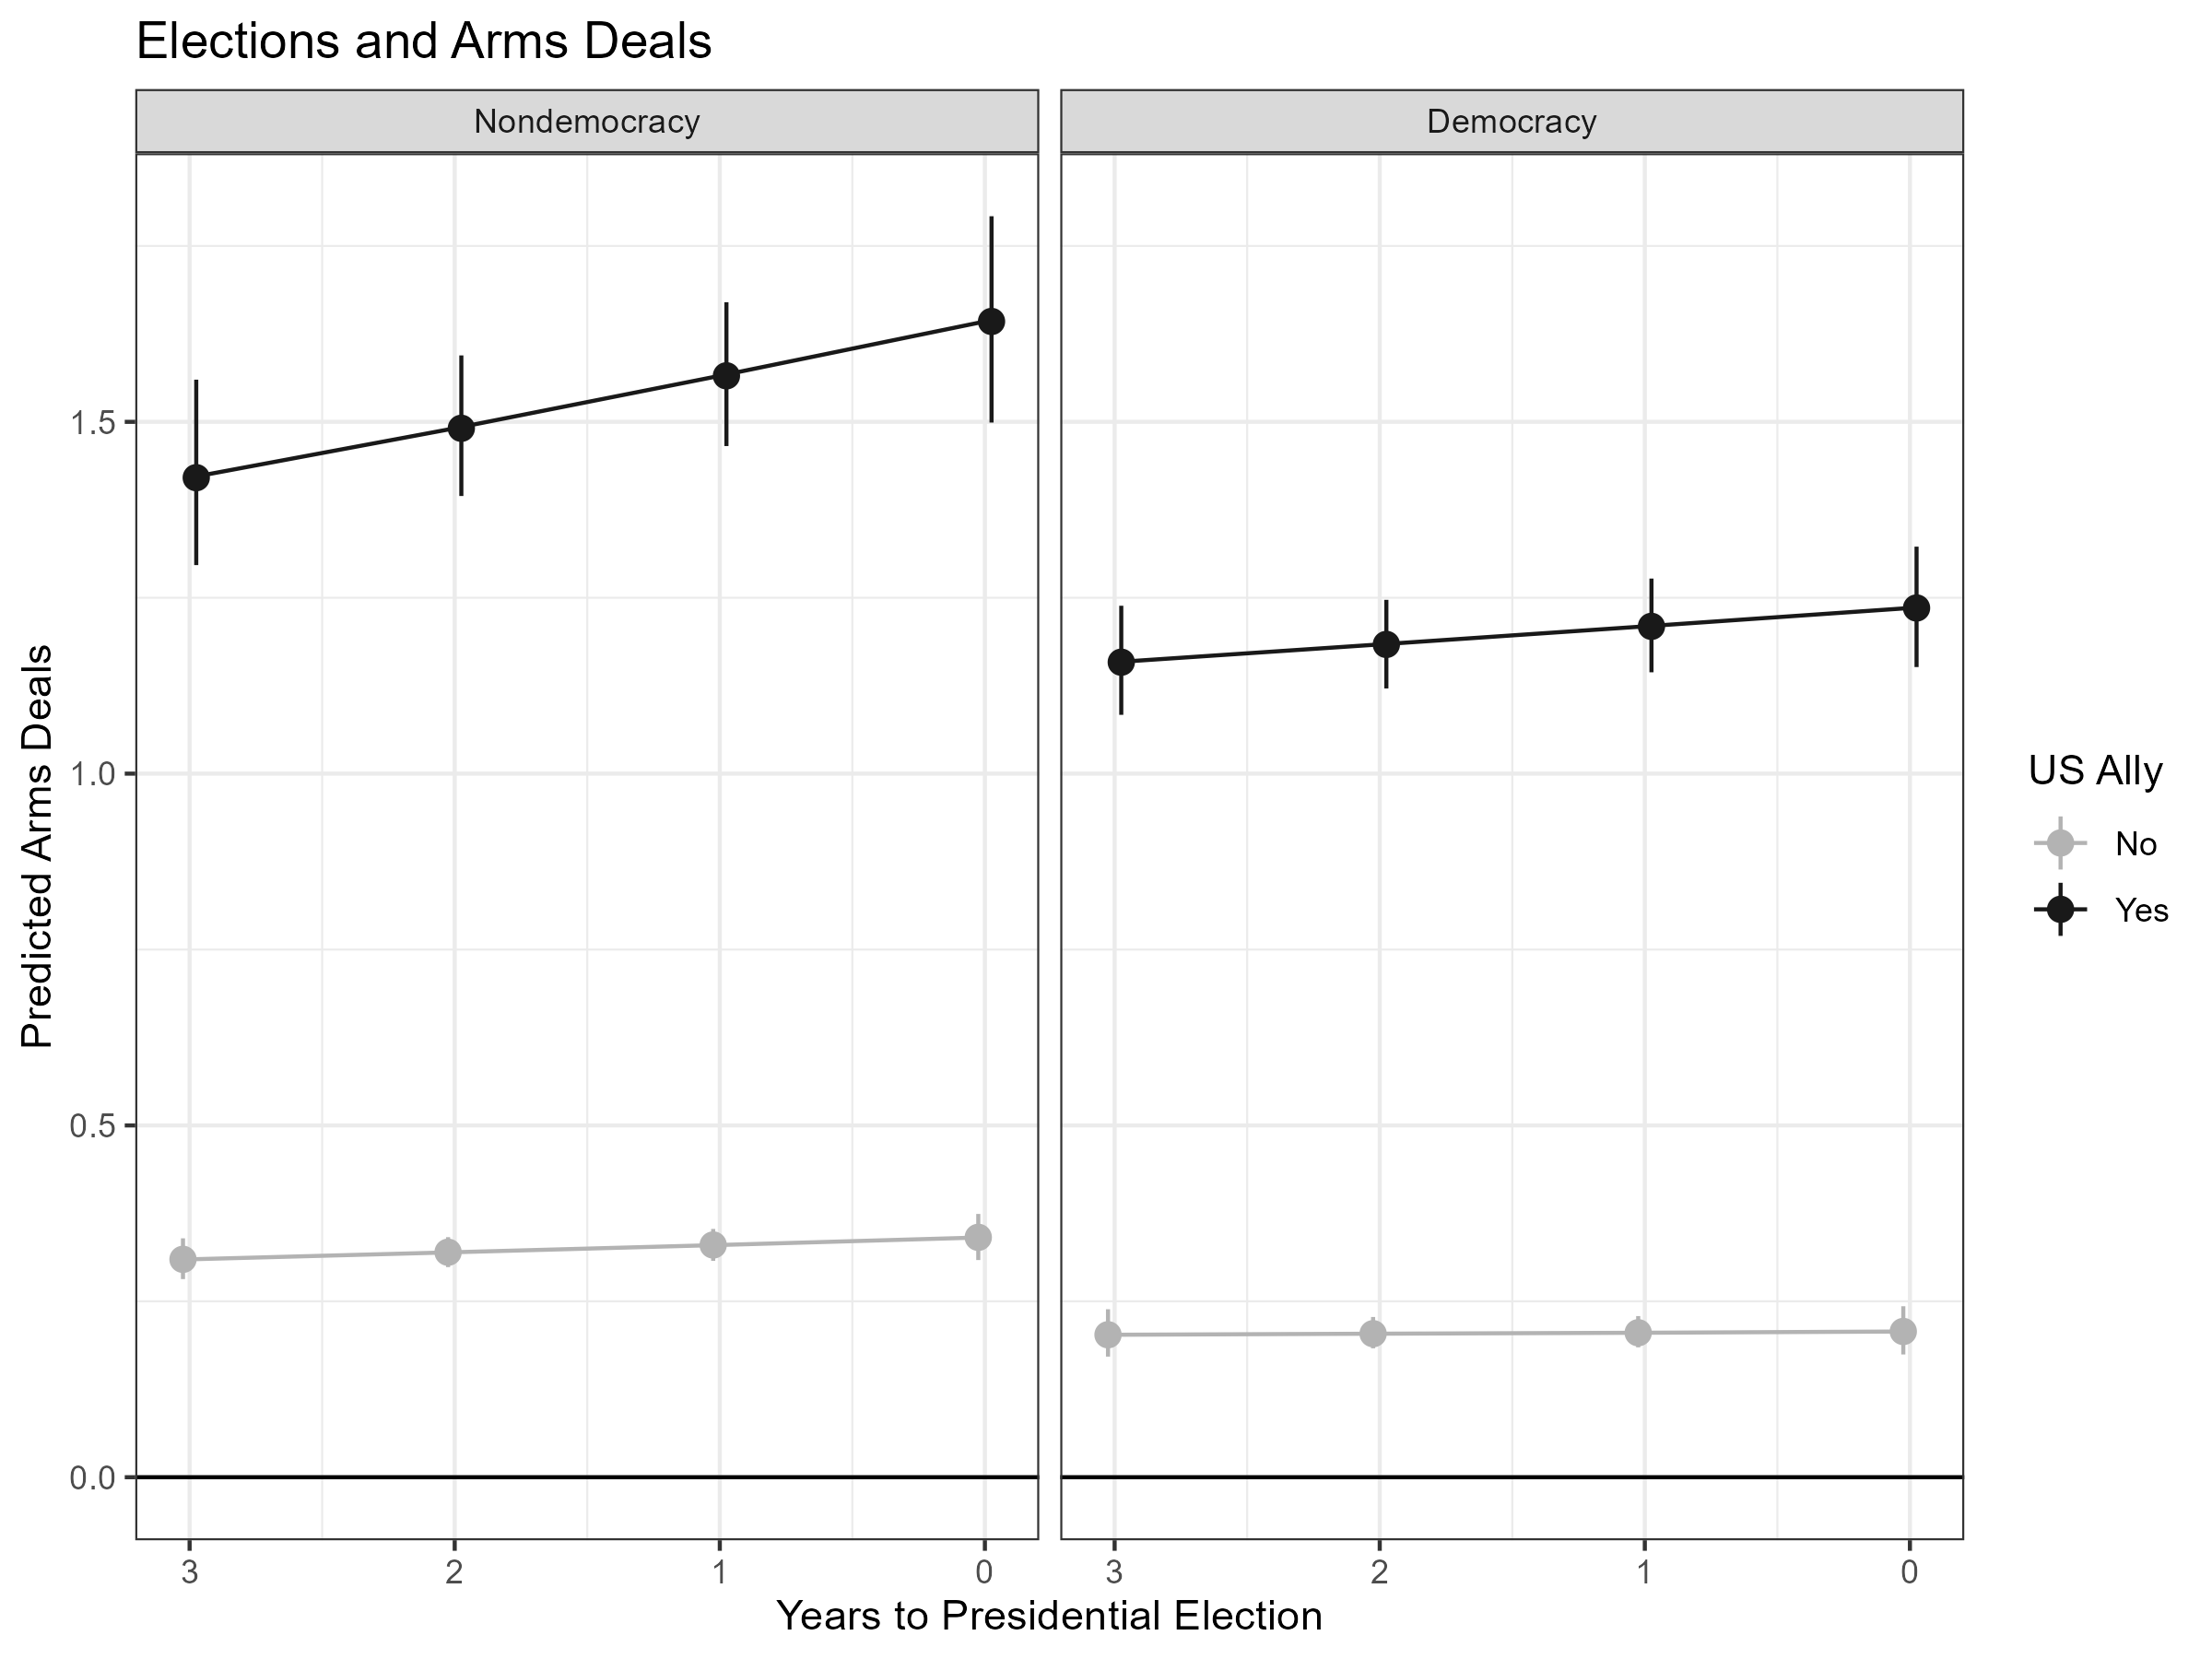
\includegraphics[width=0.95\textwidth]{../figures/us-arms-plots.png}
	\caption{Predicted arms deals between the United States and other states 1950 to 2014 based on presidential election proximity, democracy, and security alliances. Estimates derived from a hurdle Poisson model. Points mark the estimates and error bars summarize the 90\% credible interval.}
	\label{fig:us-arms-plots}
\end{figure}


The estimates in \autoref{fig:us-arms-plots} suggest that alliances facilitate arms deals with autocracies.
The United States makes more arms deals with allied states than non-allied states, regardless of partner regime. 
Predicted deals with non-allied states are much lower across all levels of democracy. 


There are cycles in arms deals in autocracies with and without a US alliance, but the cycles are much larger for allied states. 
When allied polyarchy is at the minimum, predicted arms deals rise from 2.3 to 2.7 throughout the presidential election cycle.
Hypothesis tests of equality between allied arms deals at minimum democracy at each level indicate a clear increase of .13 deals in each year of the electoral cycle.\footnote{The 90\% credible interval ranges from .05 to .21.}
The electoral cycles when democracy is at the 1st quartile or median are also clearly positive, but smaller.
Non-allied states with a minimal polyarchy score see predicted deals increase by roughly .05 a year.


Unlike autocratic allies, democratic allies receive consistent arms deals. 
Defense industrial integration may explain some of the democratic stability \citep{Brooks2005}, but another plausible explanation is that democratic leaders face more constraints on syncing deals to the presidential election cycle.
The constraint argument is also plausible because democracies make fewer arms deals overall. 


Electoral cycles are strongest for autocratic allies. 
Alliances increase the level of arms deals, and autocracies are more responsive to presidential elections. 
This suggests that autocracies with political flexibility and security motivation make electorally-driven deals that feed swing state contracts. 
In the next section, I use specific defense industrial sectors to check the connection between deals and contracts. 



\subsection{Which Weapons Drive Deals and Contracts?} 


The final analysis examines whether the weapons systems that change hands in US arms deals with autocratic allies and are correlated with swing-state contract awards. 
Showing that the United States makes more deals for specific weapons as elections approach, and that deals for those weapons are correlated with defense contract awards in swing states increases confidence in the theoretical process. 
Aircraft are the most common subject of arms deals with autocrats near elections, and aircraft deals also increase swing state contracts for aircraft production.\footnote{These correlations do not establish exact linkages between deals and specific contracts, however.}


To analyze deals by sector, I fit the models of arms deals and defense contracts with the interaction of alliance, regime type and election timing, but divided deals and contracts into six sectors. 
The six sectors include aircraft, arms and munitions, military electronics, missiles and space technology, ships, and vehicles.  
Each of these sectors has a distinct production geography and arms deal dynamics.


In the deals analysis of the the different sectors, I fit six hurdle Poisson models, one each type of arms deals. 
These models use the same covariates as the preceding arms deals model; a triple interaction of alliance, democracy and election timing, along with a series of controls and a hurdle equation.
Using the hurdle again improves model fit, as more country-year observations have zero deals within sectors. 


For ease of presentation, I plot predicted arms deals at the minimum and maximum of partner democracy in \autoref{fig:deals-sector}.
The estimates suggest that aircraft are the core weapons system in electoral cycles in arms deals with autocratic allies. 
Military alliances strongly increase the likelihood of arms deals for aircraft and regime type determines whether aircraft deals follow presidential election cycles. 
Aircraft deals with autocratic allies are the most common deal overall, and these deals rise as presidential elections approach. 
While aircraft deals with democratic allies are also common, they are less responsive to election timing. 



\begin{figure}[htpb]
	\centering
		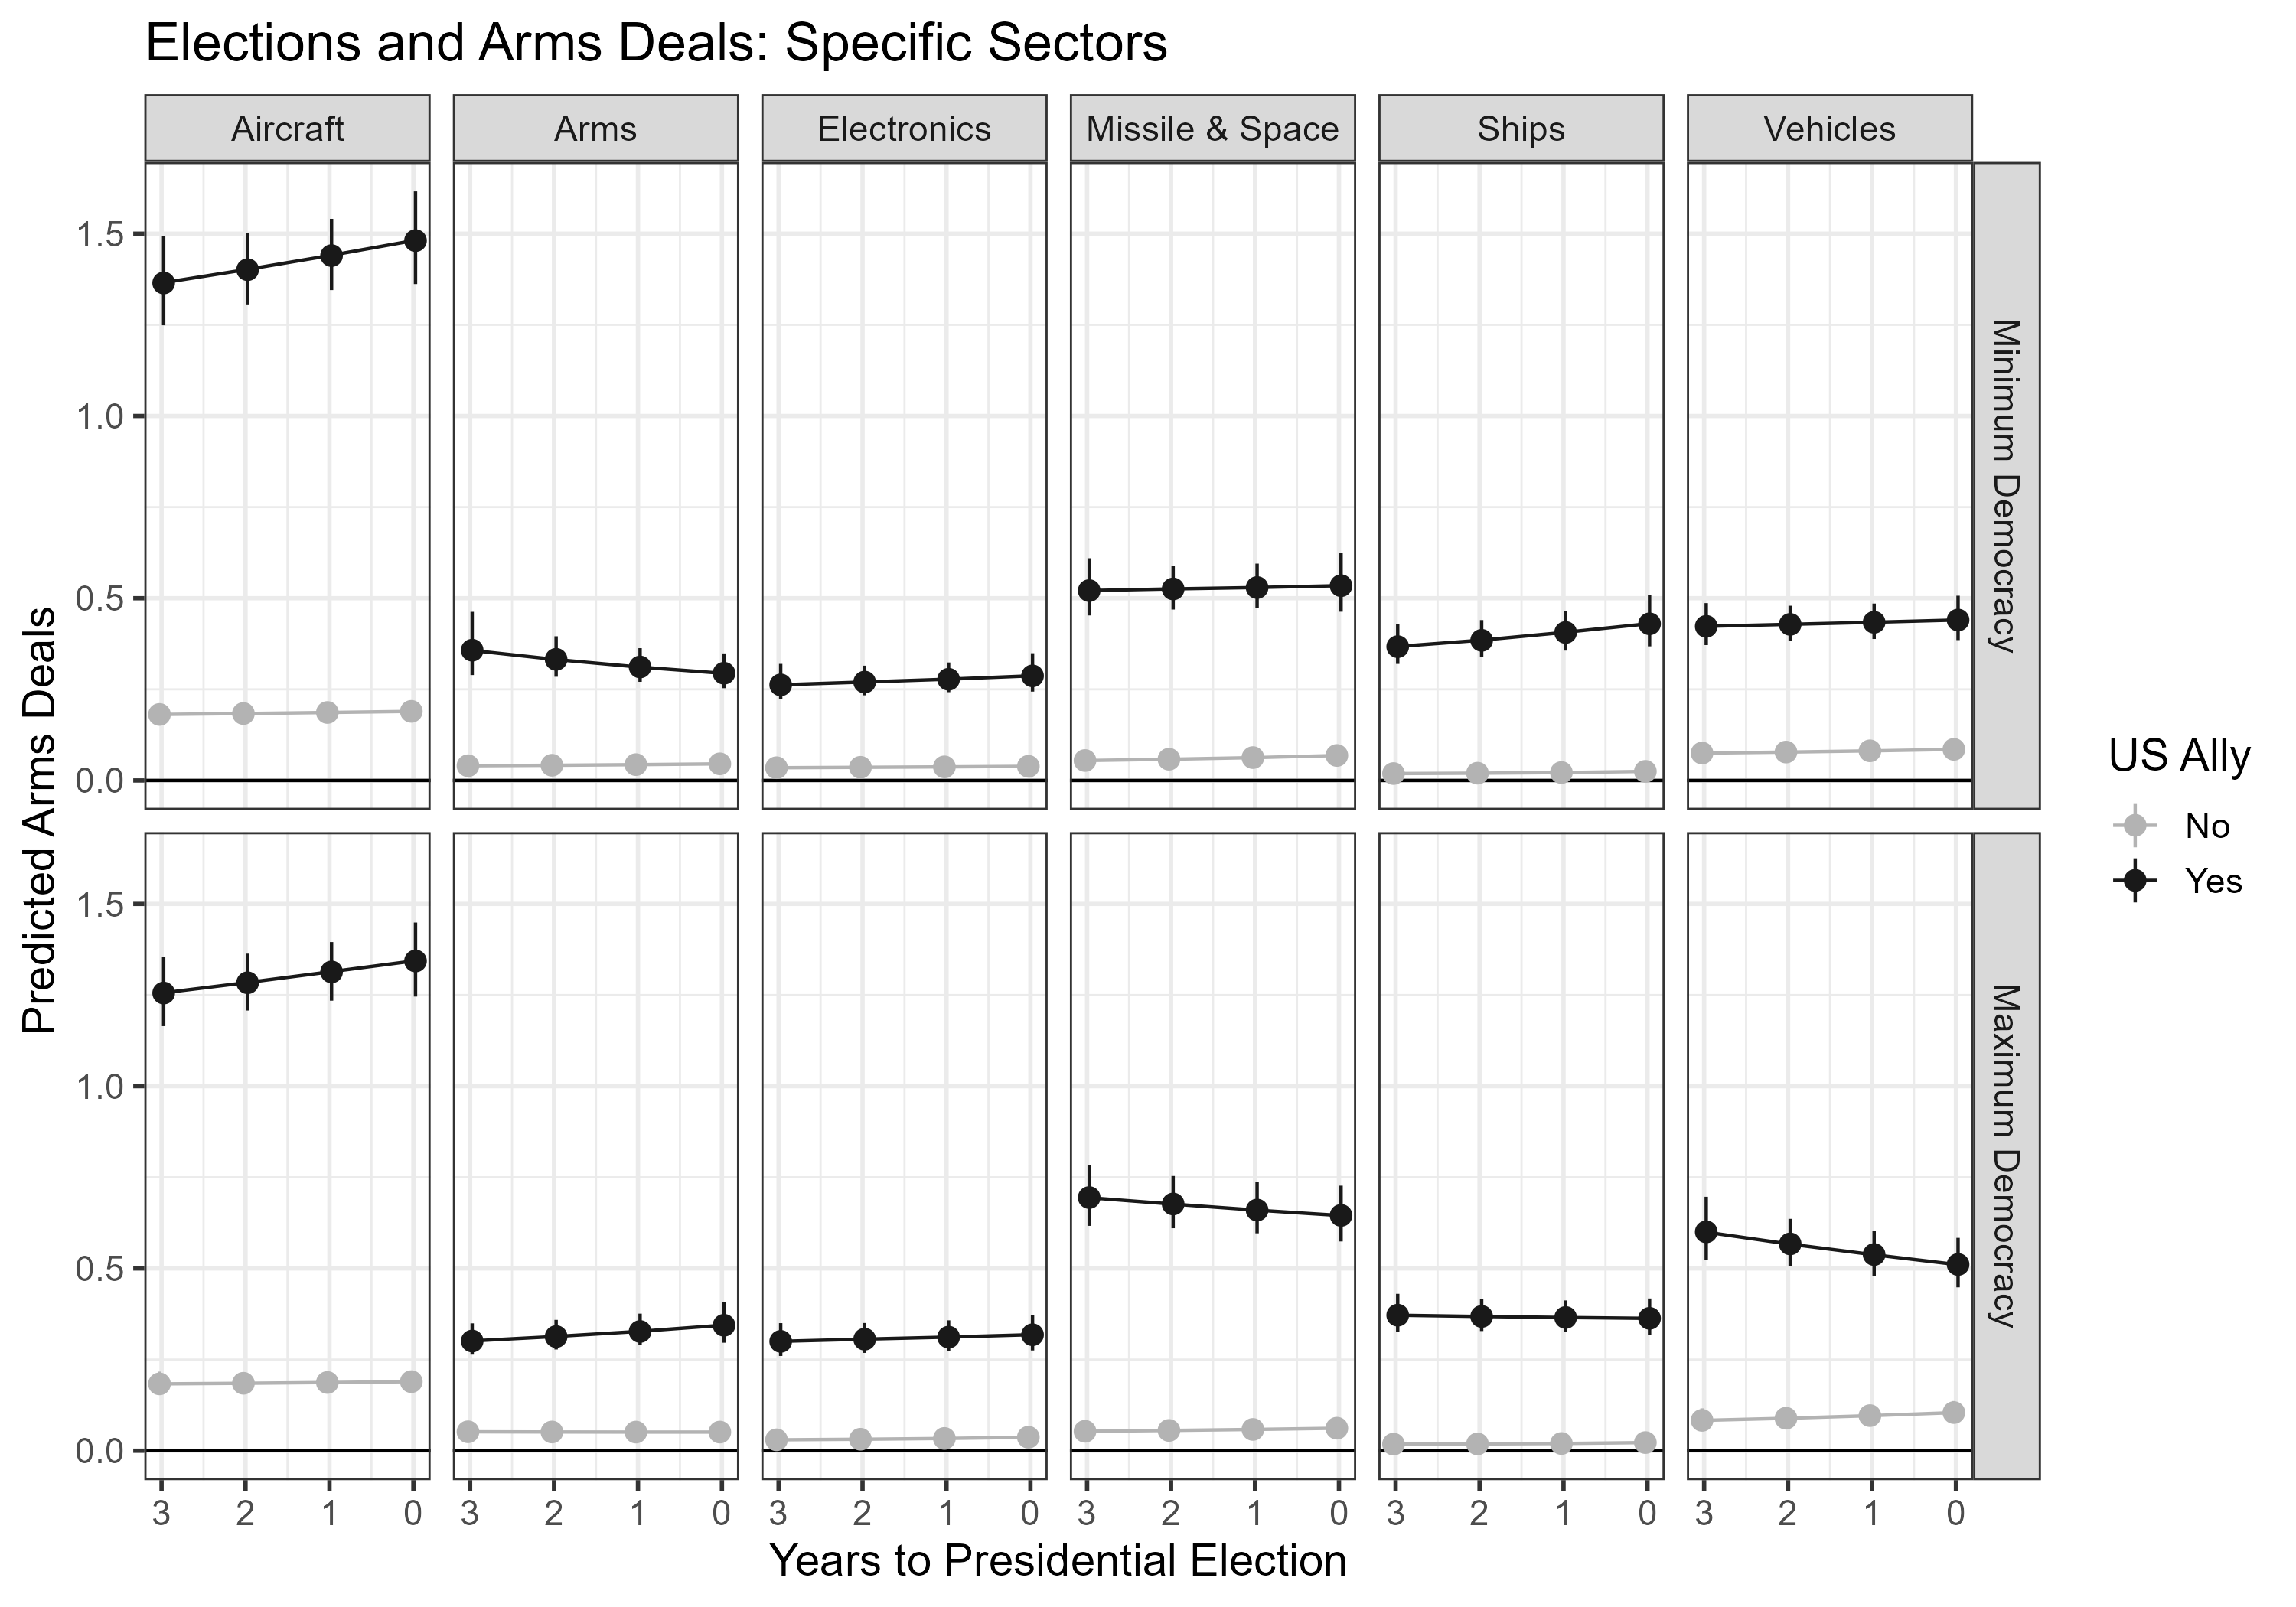
\includegraphics[width=0.95\textwidth]{../figures/deals-sector.png}
	\caption{Predicted arms deals between the United States and other states 1950 to 2020 based on presidential election proximity, democracy, and military alliance. Estimates derived from six sector-specific hurdle Poisson models counting annual deals divided by the type of military good exchanged. Points mark the estimates and error bars summarize the 90\% credible interval.}
	\label{fig:deals-sector}
\end{figure}


Among autocracies, alliances increase deals for ships, and ship deals increase with electoral proximity. 
Allies make more ship deals at all levels of democracy, but only autocratic allies make more deals near elections. 
Ships could also contribute to efforts to use arms deals to feed defense contracting. 


Other weapons show less evidence of cycles in arms deals. 
Deals for arms and other munitions do not depend on democracy or election timing. 
Democratic allies are more likely to make deals for military electronics and missile/space systems. 
The importance of democracy and alliances for these goods likely reflects trade in intermediate goods to support joint production, as well as joint operations in NATO and other U.S. alliances. 


%Neither electronics nor missile and space systems see electoral deal cycles.
%Deals for military vehicles do not track the electoral cycle either. 
%Among autocracies, alliances make no difference for vehicle deals. 
%Allied democracies see small decreases in deals as elections approach. 


To examine the deals and contracts hypothesis for each sector, I also fit six models of defense contracts. 
This analysis divides total contracts by sector using the product description for each contract. 
As in the analysis of aggregate defense contracting, I rescale the outcome between 0 and 1 using the annual sum of contracts for those defense goods. 
I then fit ordered beta regression models of the rescaled outcomes, using an identical specification to the aggregate defense contracting model.
The key independent variables in these models are observed arms deals in each sector, the binary swing state indicator, and their interaction. 
I also include terms to capture state varying intercepts, state-specific autocorrelation, and other controls. 


Aircraft deals are strongly correlated with contracts for military aircraft in swing states. 
\autoref{fig:me-deals-sector} plots the interaction between different deal types and swing state status.  
These estimates show the deals coefficients from six ordered beta models, transformed back on the outcome scale. 
Again, I focus on the positive posterior mass, as this shows the extent of evidence consistent with a directional hypothesis more clearly than credible intervals.


\begin{figure}[htpb]
	\centering
		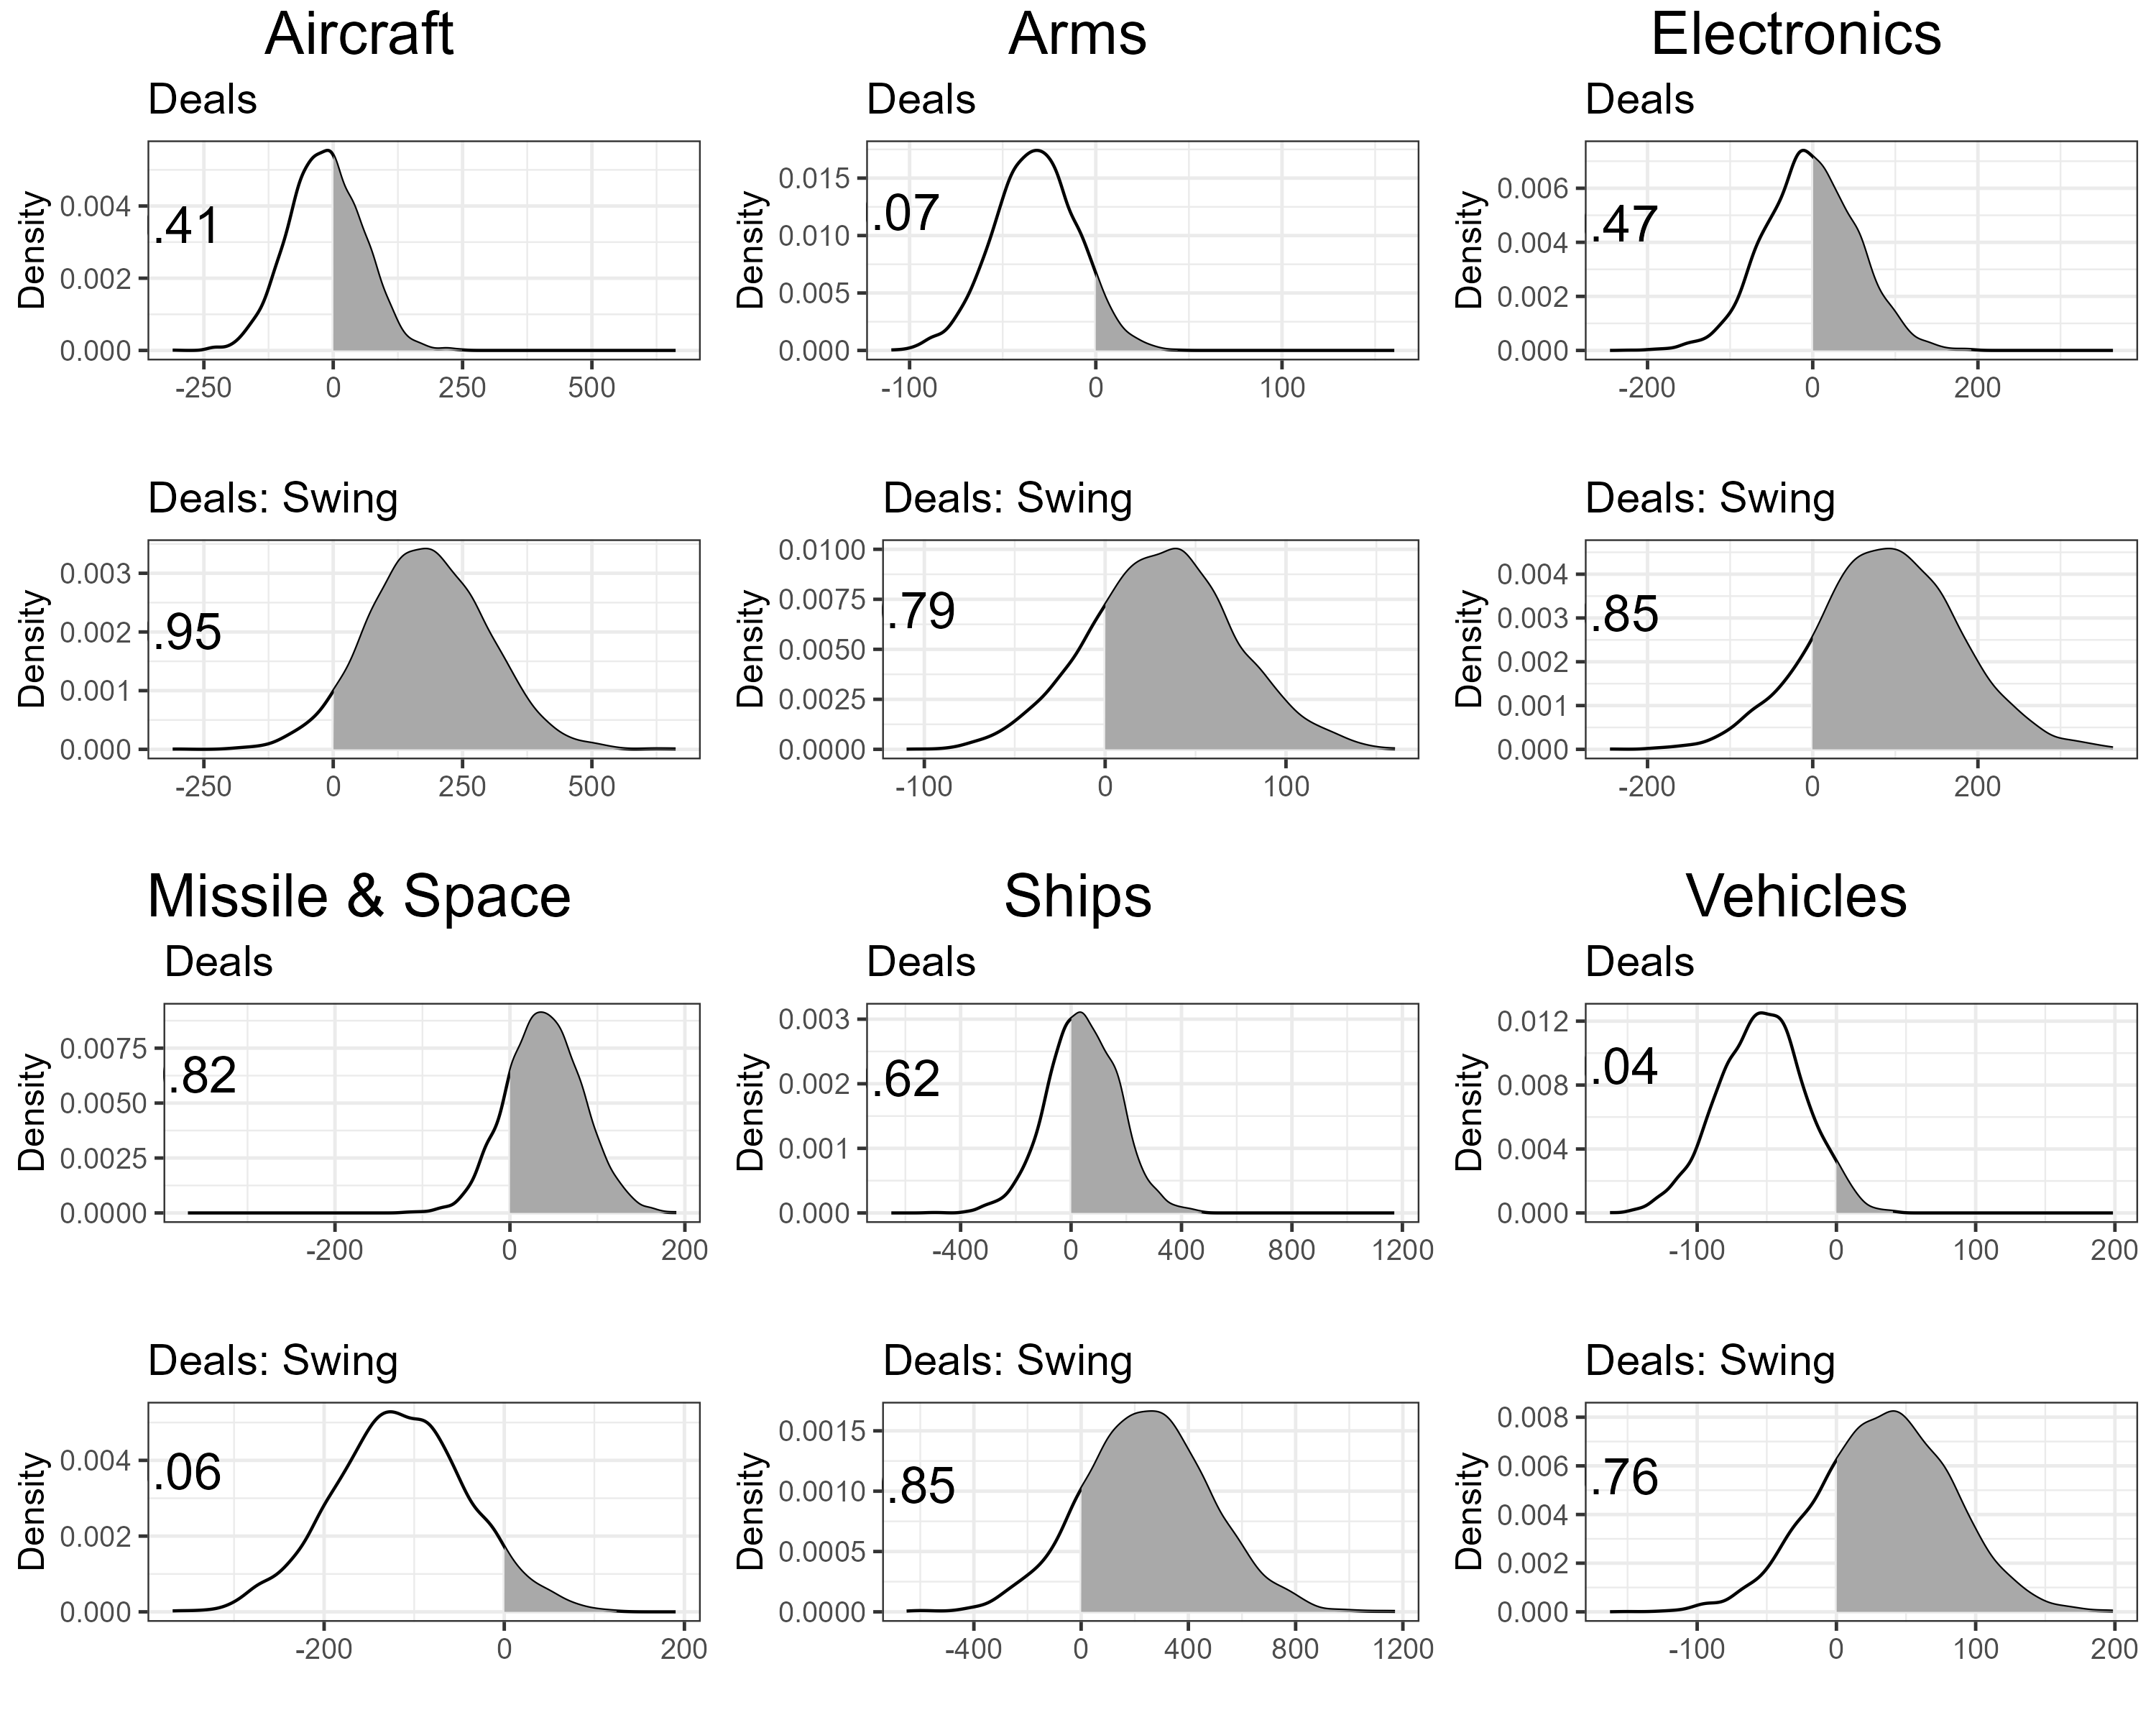
\includegraphics[width=0.95\textwidth]{../figures/me-deals-sector.png}
	\caption{Associations between different types of arms deals on corresponding defense contracts. Shaded are and text summarize the positive posterior mass. Estimates in millions of US dollars.}
	\label{fig:me-deals-sector}
\end{figure}


While deals for most systems like arms, vehicles, and missile and space components have largely positive associations with swing state contract awards in their sector, aircraft deals have a large and overwhelmingly positive association. 
95\% of the posterior mass in the interaction of aircraft deals and swing state status is positive.
This reflects the diffuse aircraft supply chain for aircraft, which orders for engines, airframes, and other essential goods. 


In addition to aircraft, ships and electronic deals are largely associated with greater swing state contracts. 
Increases in ships deals are associated with \$300 million more contracts in a hypothetical swing state. 
Annual ships deals range from one to 11, so these deals are rare but potentially lucrative. 
The impact also may not concentrate in shipyards, as most ships deals cover whole platforms, which require components from other regions. 

 
While electronics deals are less cyclical, most of the association between electronics deals and swing state contracts for military electronics is positive as well.
Electronics manufacturing does not come from arms deals with autocratic allies, but these deals also feed swing state contracts. 
Similarly, much of the vehicles posterior mass is positive in swing states, though the direction of that association is less clear. 
Only missile and space production, which is very geographically concentrated, has greater positive mass on the association between deals and contracts outside of swing states.


These results suggest that aircraft are the main component in arms deal cycles and aircraft deals often increase swing state contracts. 
Other deals in sectors like arms, electronics and ships may also increase swing state contracts, but these have less cyclical arms deals. 
These estimates suggest that there is a connection between arms deals with autocratic allies and swing state contracts.  



\section{Discussion and Conclusion}


Arms deals with autocratic allies help U.S. leaders increase defense contracting awards in swing states. 
Arms deals with autocracies increase as presidential elections approach and deals also increase swing state contract awards. 
Much of this cooperation sends aircraft to autocratic allies like the Brazilian junta and Saudi Arabia.


% alliance value and autoc alliance durability
This note helps explain U.S. allies with autocracies endure despite normative and practical criticisms. 
Arms deals increase autocratic allies' security and help U.S. leaders win elections.
While not a part of formal alliance terms, these informal linkages are essential to grand bargains between alliance patrons and prot{\'e}g{\'e}s.
%Allies need not undertake these cycles deliberately, but making arms deals is part of a cooperative bundle of ties.


In addition to adding a new explanation for security cooperation with autocracies, these findings add an international security component to the political budget cycle literature.
Alliance partnerships can help leaders manipulate economic conditions for electoral gain. 
By providing an outlet for defense contracting, allies help leaders award contracts with less attention to the absorptive capacity and force planning of the U.S. military.


The argument and findings also complement prior findings that states manipulate international economic and security cooperation to bolster or undermine leaders \citep{ChyzhUrbatsch2021, KimMargalit2021}. 
Some allies have both motive and means to use security cooperation to help leaders. 
Allied arms deals sustain regular cooperation across regimes.


Future research could proceed in several directions. 
Exploring the role of defense industry integration and intermediate goods in these arms cycles is critical.
Whether there are similar cycles outside the United States is also a worthy subject of future study. 
Other alliance patrons may take similar actions in different industries, for instance.


Electoral competition reshapes international security cooperation.
Efforts to use defense contracting to improve the economy in swing states encourage arms deals with autocratic U.S. allies.
While these deals may empower states that misuse U.S. arms, electoral considerations take precedence. 


\newpage
\singlespace
 
\bibliography{../../MasterBibliography} 


\end{document}
